%priprava posamezne ure
%tukaj zaporedoma napisemo{st. zaporedne ure}{datum}{naslov}{poglavje}{oblika dela}{pripomocki}
\begin{priprava}{}{}{Kombinatorika}{Kombinacije}{frontalna}{tabla}

Uvodna motivacija: Pika Nogavička ima 5 različnih nogavic. Koliko parov lahko izbere od njih?

\begin{figure}[h]
    \centering
    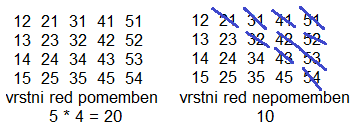
\includegraphics[width=0.5\textwidth]{slike/kombinacije1.png}
\end{figure}

\textcolor{red}{\textbf{Kombinacija reda $ r $ med $ n $ elementi} = razporeditev $ n $ različnih elementov na $ r $ mest, kjer \emph{vrstni red ni pomemben}.}
Število teh razporeditev običajno označimo z $ C^r_n $.

\didopomba{Na to lahko gledamo kot variacije -- $ n $ elementov razporejamo na $ r $ mest, ker pa vrstni red ni pomemben, delimo še s številom mest, tj. $ r \rightarrow $ intuitivno pridemo do formule in uvedemo tisto oznako ``n nad r'' = ``od n izbereš r'':}
$$ C^r_n = \frac{V^r_n}{r!} = \frac{n!}{(n - r)! r!} = \binom n r $$

\vaje{
Vaje:
\begin{itemize}
    \item par enostavnih vaj iz binomskega simbola. \didopomba{lahko ugotovimo, da $ r $ pove, koliko členov vzamemo v produktu v števcu: $ \binom {100} 3 = \frac{100 \cdot 99 \cdot 98}{3!} $, ampak to ni za se napiflat!}
    \item Zapiši potenčno množico množice $ \mathcal{A} = {a, b, c, d} $. Koliko je podmnožic s tremi elementi? Koliko je vseh podmnožic?
    \item Primeri z vlečenjem kroglic iz škatlic, parov ljudi \ldots
\end{itemize}
}

\textbf{Lastnosti binomskih simbolov} \didopomba{napišeš in sami dokažejo}
\begin{itemize}
    \item $ \binom n 0 = 1 $
    \item $ \binom n n = 1 $
    \item $ \binom n 1 = n $
    \item $ \binom n r = \binom n {n - r} $
    \item $ \binom n r + \binom n {r + 1} = \binom {n + 1} {r + 1} $ \didopomba{tukaj je še dokaz s slikco in premislekom v levo stran: od $ n + 1 $ elementov lahko izberemo $ r + 1 $ tako, da osamiš en element in od $ n $ izbereš $ r + 1 $ ALI pa izbereš tistega osamljenega in od $ n $ izbereš še $ r $ elementov.}
\end{itemize}
    
\end{priprava}